  \pagebreak
  \section{Actividad Práctica}
    Se propone como actividad realizar el análisis de distintas señales en la frecuencia con el uso del
    módulo matemático de un osciloscopio digital, mediante la FFT. Con este objetivo, los instrumentos
    e insumos necesarios son:

    \begin{itemize}
      \item Osciloscopio digital Tektronix TDS 1001
      \item 2 generadores de señal Goldstar FG-8002
      \item Multímetro Unit UT890C
      \item Circuito modulador de amplitud con diodo y circuito sintonizado
      \item Potenciómetro de $1~k\Omega$
      \item Amplificador transistorizado de dos etapas
    \end{itemize}

    \input{Secciones/Subsecciones/1AnalisisDeUnaSeñalCuadrada.tex}
      \subsection{Análisis de un tren de pulsos}

    Se analiza a continuación una señal con forma de onda de tren de pulsos rectangulares, en el dominio 
    de la frecuencia.
    Se sabe que la relación de período en el dominio del tiempo y ancho de banda en el dominio de la frecuencia, 
    es inversamente proporcional. Es por ello, que se utiliza una señal de pulsos rectangulares, para poder visualizar 
    dicha relación.

    Se configura el generador de la siguiente manera: período de $\mathbf{1~ms}$, ancho de pulso de 
    $\mathbf{250~} \boldsymbol{\mu} \mathbf{s}$, y se gira media vuelta la perilla de control de amplitud.
    El ajuste del generador se observa en el osciloscopio en la Figura~\ref{fig:Exp2SeñalPulso}.

      \begin{figure}[H]
        \centering
        \begin{subfigure}[H]{0.48\textwidth}
          \frame{\includegraphics[width=\textwidth]{Imagenes/ActividadPractica/2AnalisisDeUnTrenDePulsos/Exp2_PeriodoDeLaSeñalDeEntrada.jpeg}}
          \caption{Señal pulsante de período de $1~ms$.}
        \end{subfigure}
        \hfill
        \begin{subfigure}[H]{0.48\textwidth}
          \frame{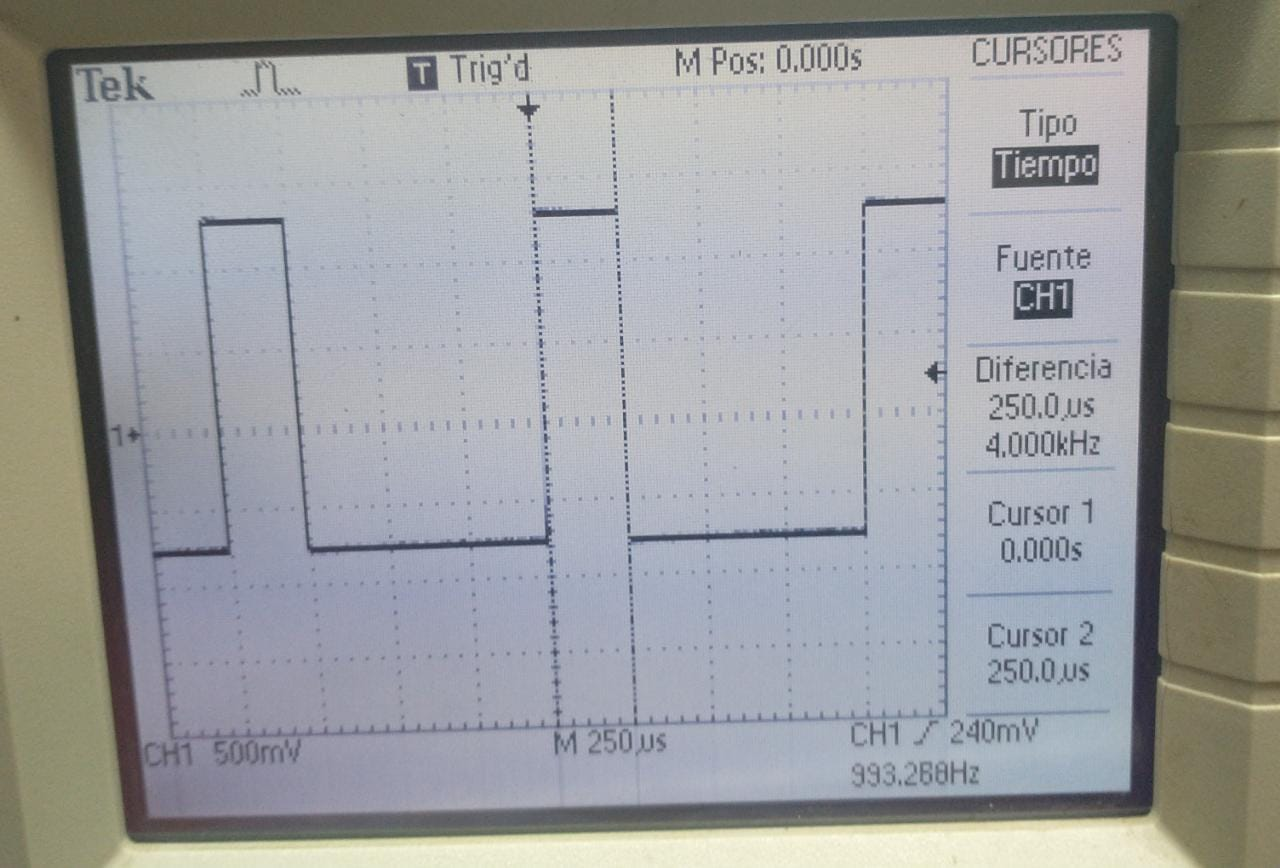
\includegraphics[width=\textwidth]{Imagenes/ActividadPractica/2AnalisisDeUnTrenDePulsos/Exp2_AnchoDelPulsoDeEntrada.jpeg}}
          \caption{Ancho del pulso de $250~\mu s$.}
        \end{subfigure}

        \caption{Tren de pulsos.}
        \label{fig:Exp2SeñalPulso}
      \end{figure}

    Ahora, se cambia al modo matemático a través del botón \textbf{MATH MENU}, y se configura con: \textbf{FFT}, 
    \textbf{CH1}, \textbf{Rectangular}, \textbf{Zoom X1} y modo adquisición \textbf{Promedio} en 64 muestras. 
    Dicha configuración se enseña en la Figura~\ref{fig:Exp2SeñalPulsanteEspectro}.

      \begin{figure}[H]
        \centering
          \frame{\includegraphics[width=0.48\textwidth]{Imagenes/ActividadPractica/2AnalisisDeUnTrenDePulsos/Exp2_EspectroDeLaSeñalPulsante.jpeg}}
          \caption{Análisis en frecuencia de la señal de entrada.}
          \label{fig:Exp2SeñalPulsanteEspectro}
      \end{figure}

      Luego, se observa cómo varía el espectro entre los 3 tipos de ventana: \textbf{Hanning}, \textbf{Rectangular}, 
      y \textbf{Flattop}, lo cual se ve en la Figura~\ref{fig:Exp2SeñalPulsanteVentanasEspectro}.

      \begin{figure}[H]
        \centering
        \begin{subfigure}[H]{0.48\textwidth}
          \frame{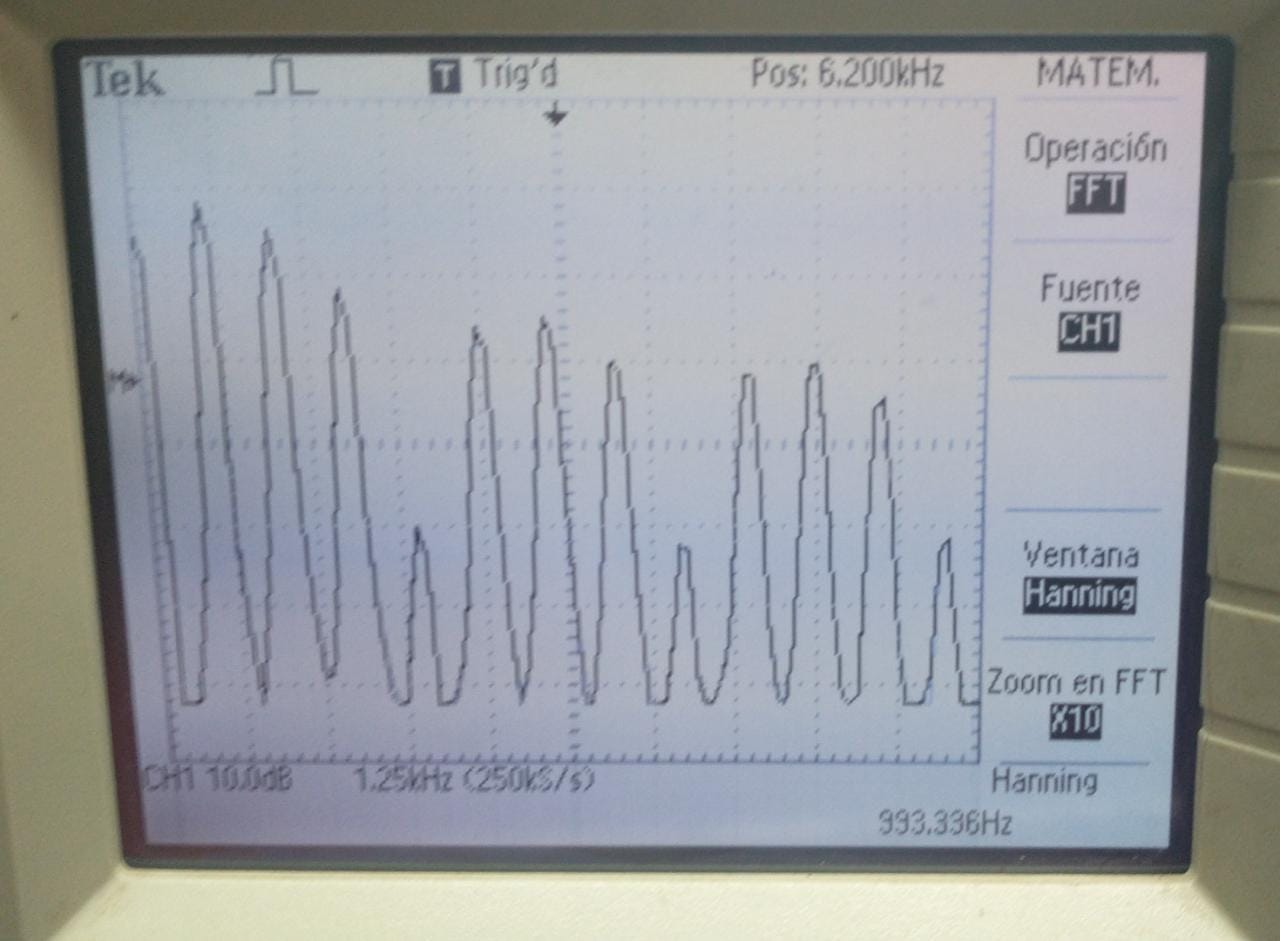
\includegraphics[width=\textwidth]{Imagenes/ActividadPractica/2AnalisisDeUnTrenDePulsos/Exp2_EspectroEnVentanaHannin.jpeg}}
          \caption{Ventana Hanning.}
        \end{subfigure}
        \hfill
        \begin{subfigure}[H]{0.48\textwidth}
          \frame{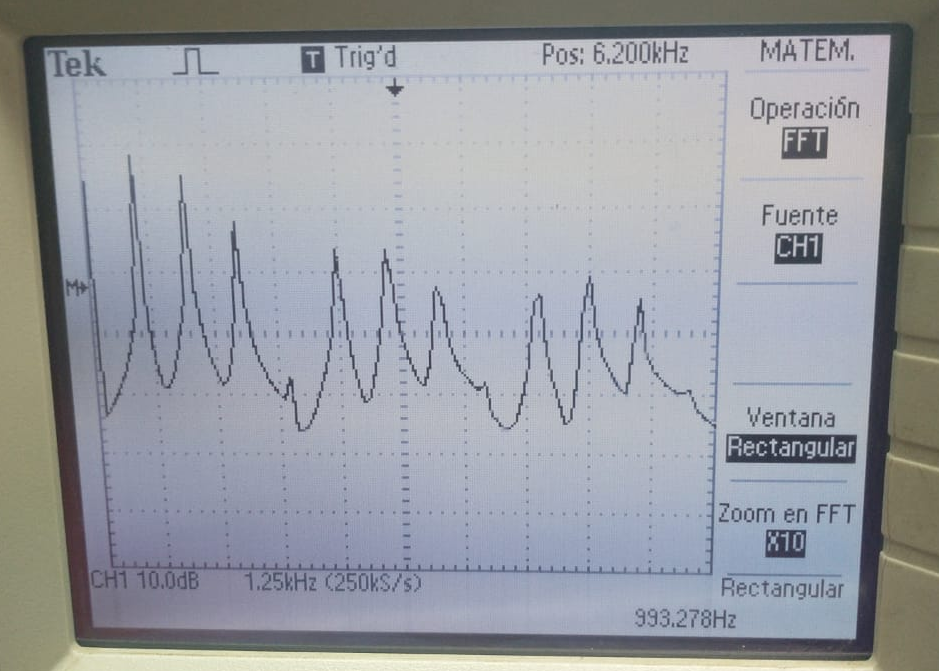
\includegraphics[width=\textwidth]{Imagenes/ActividadPractica/2AnalisisDeUnTrenDePulsos/Exp2_EspectroEnVentanaRectangular.png}}
          \caption{Ventana Rectangular.}
        \end{subfigure}
        \begin{subfigure}[H]{0.48\textwidth}
          \frame{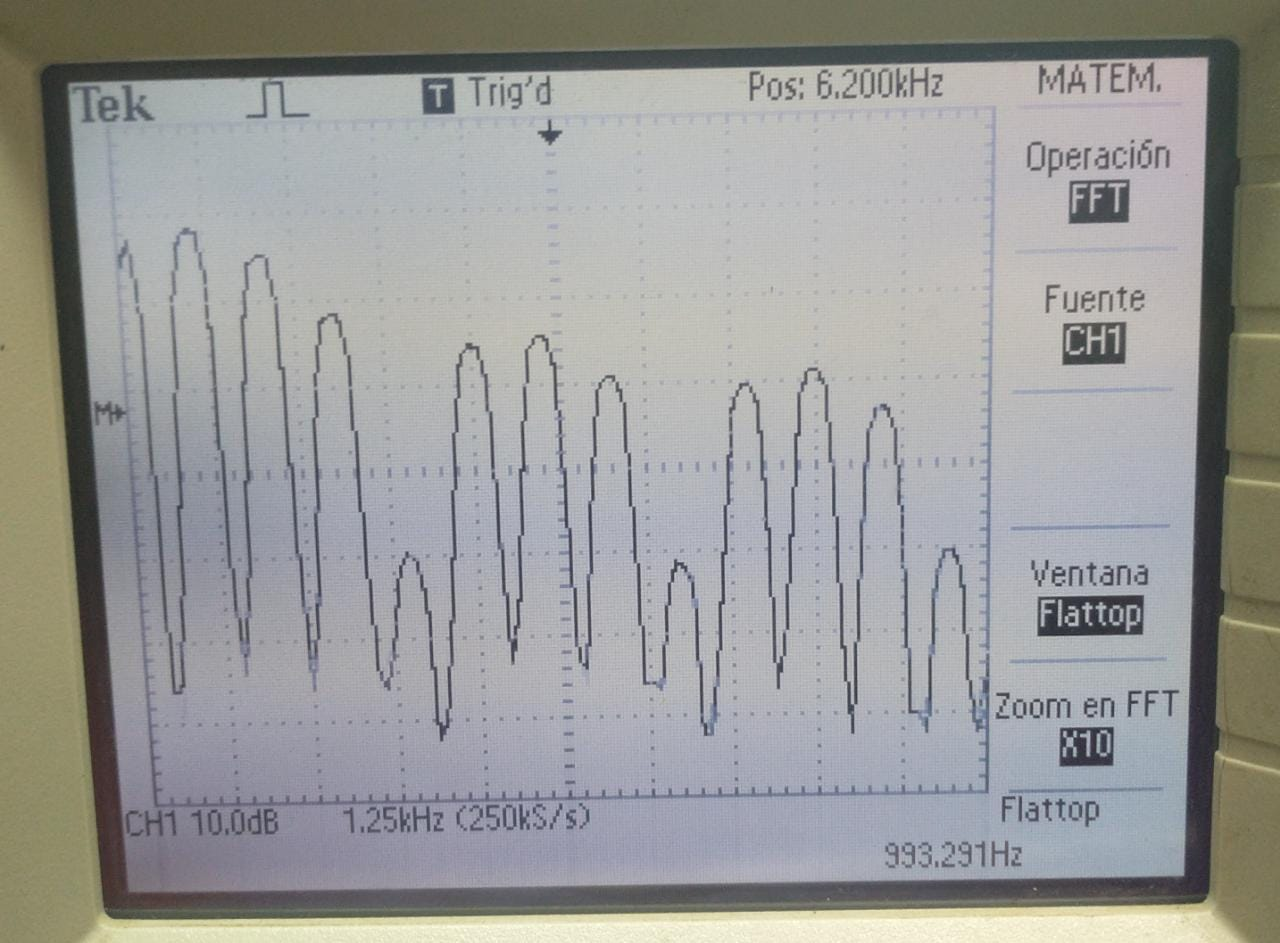
\includegraphics[width=\textwidth]{Imagenes/ActividadPractica/2AnalisisDeUnTrenDePulsos/Exp2_EspectroEnVentanaFlattop.jpeg}}
          \caption{Ventana Flattop.}
        \end{subfigure}

        \caption{Análisis en frecuencia con las distintas ventanas.}
        \label{fig:Exp2SeñalPulsanteVentanasEspectro}
      \end{figure}

      A continuación, se selecciona ventana \textbf{Rectangular}, se coloca el menú de cursores, y se selecciona 
      \textbf{frecuencia} en fuente 
      \textbf{Matemático}. Se coloca el \textbf{Cursor 1}, en $0~Hz$ y con el \textbf{Cursor 2} se 
      procede a medir las frecuencias de cada pico, como muestra la 
      Figura~\ref{fig:Exp2SeñalPulsanteArmonicosEspectro}.

       \begin{figure}[H]
        \centering
        \begin{subfigure}[H]{0.48\textwidth}
          \frame{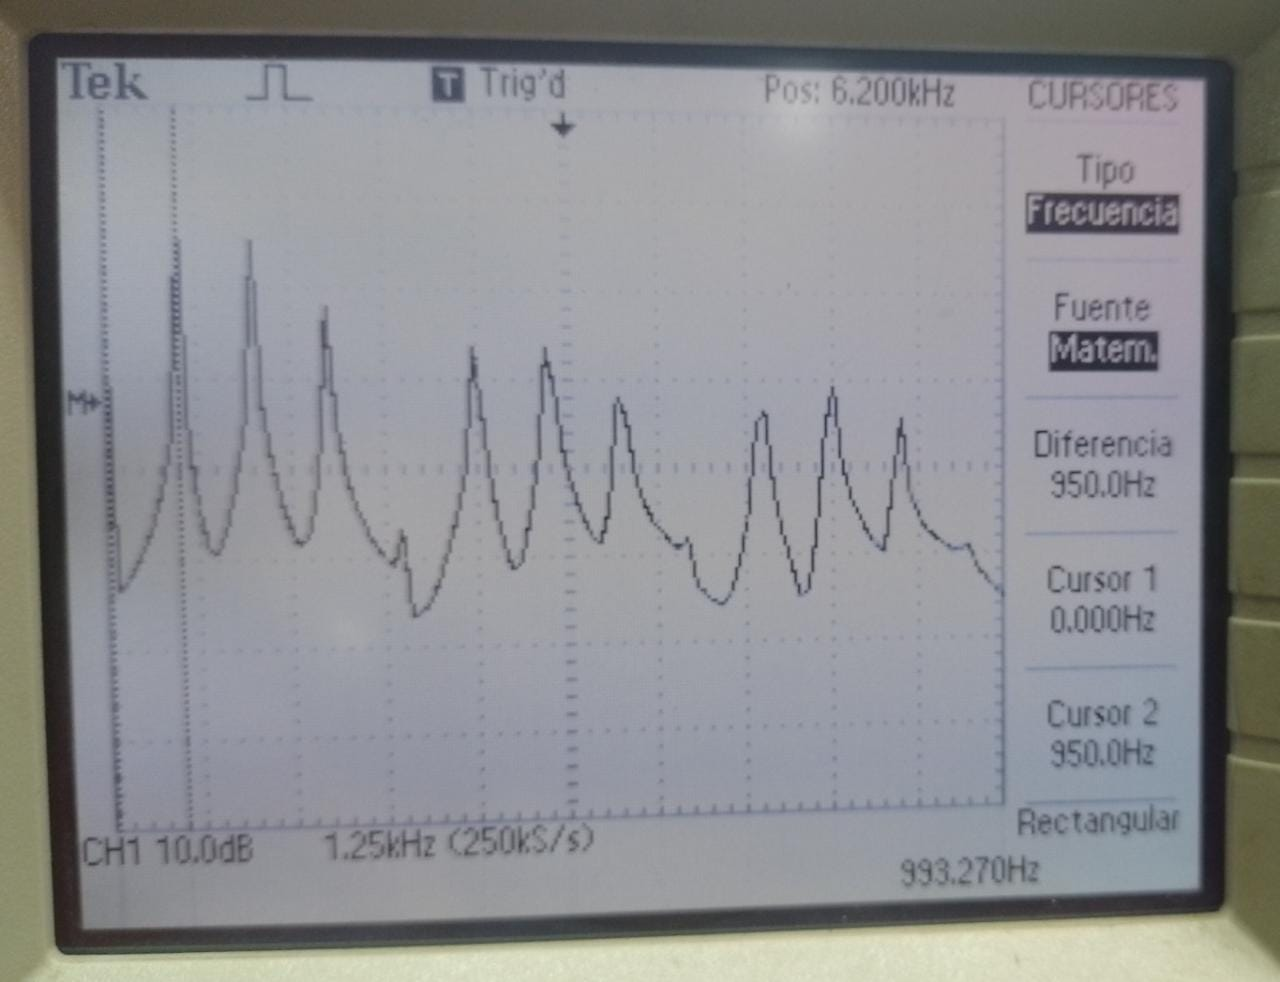
\includegraphics[width=\textwidth]{Imagenes/ActividadPractica/2AnalisisDeUnTrenDePulsos/Exp2_FrecArmonico1.jpeg}}
          \caption{Frecuencia de la fundamental en ventana Rectangular, $f_{1}=950~Hz$.}
        \end{subfigure}
        \hfill
        \begin{subfigure}[H]{0.48\textwidth}
          \frame{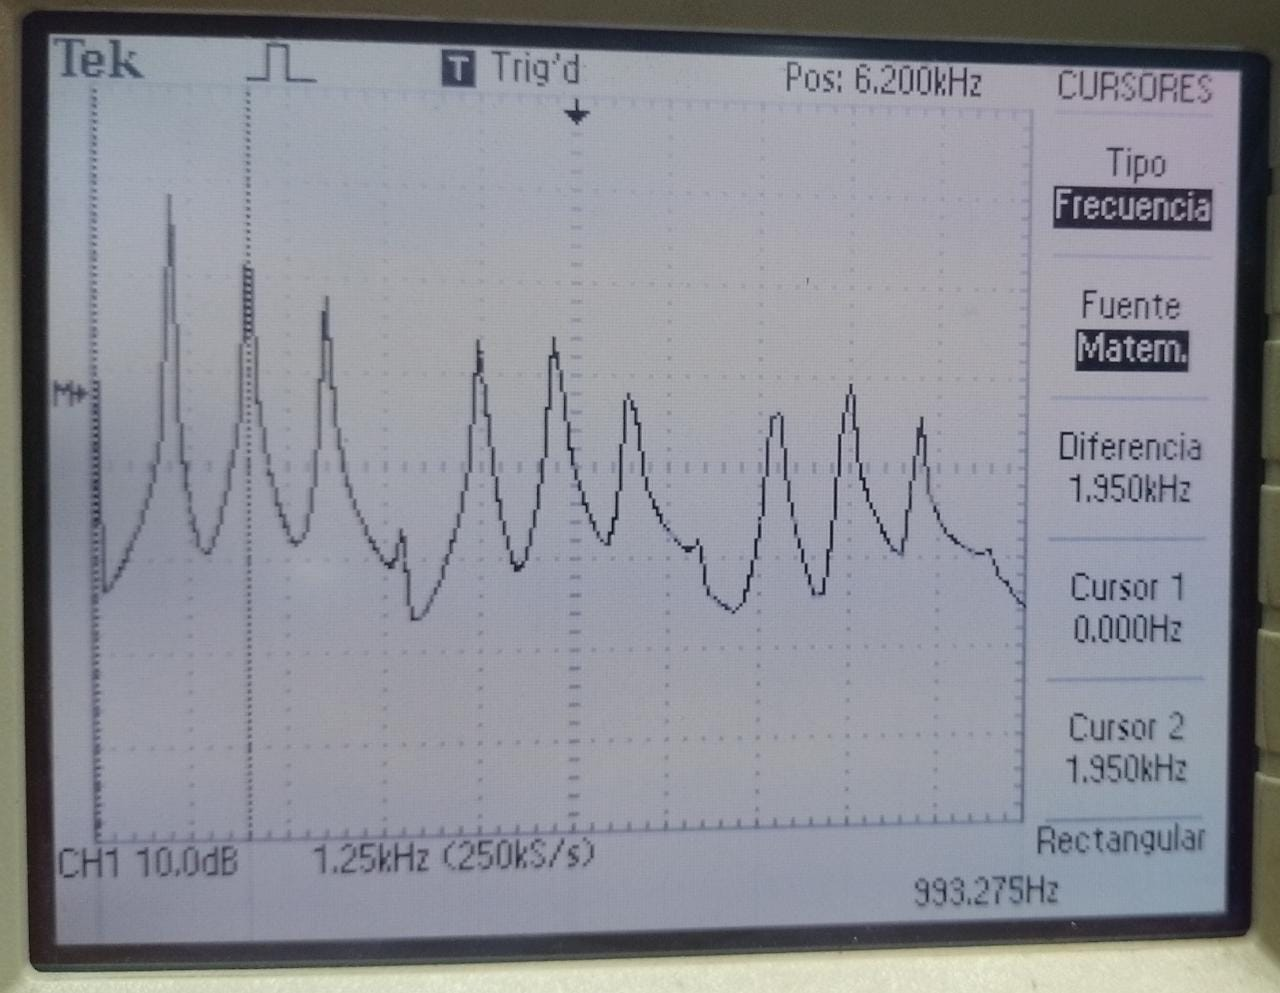
\includegraphics[width=\textwidth]{Imagenes/ActividadPractica/2AnalisisDeUnTrenDePulsos/Exp2_FrecArmonico2.jpeg}}
          \caption{Frecuencia de la segunda armónica en ventana Rectangular, $f_{2}=1950~Hz$.}
        \end{subfigure}
        \begin{subfigure}[H]{0.48\textwidth}
          \frame{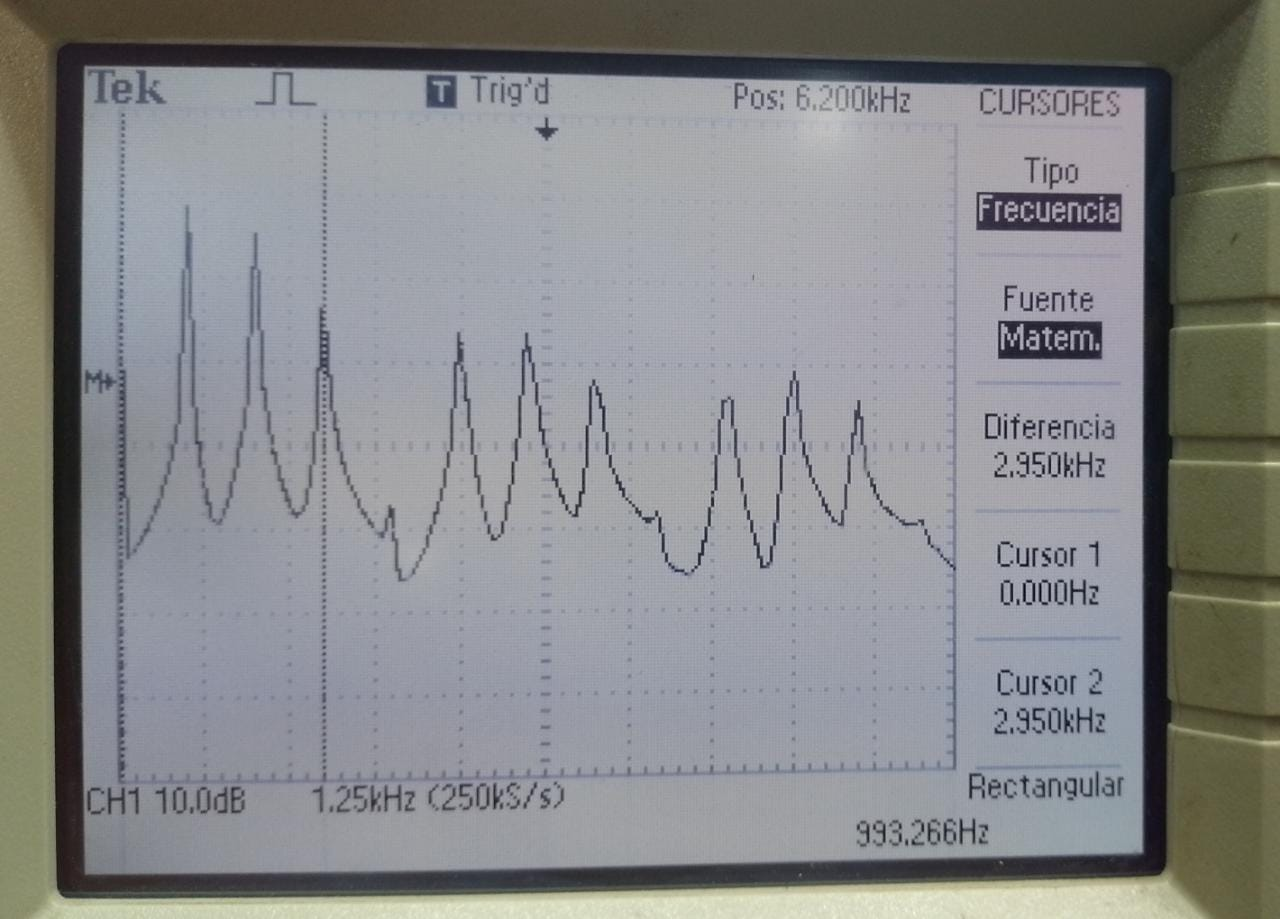
\includegraphics[width=\textwidth]{Imagenes/ActividadPractica/2AnalisisDeUnTrenDePulsos/Exp2_FrecArmonico3.jpeg}}
          \caption{Frecuencia de la tercera armónica en ventana Rectangular, $f_{3}=2950~Hz$.}
        \end{subfigure}
       \hfill
        \begin{subfigure}[H]{0.48\textwidth}
          \frame{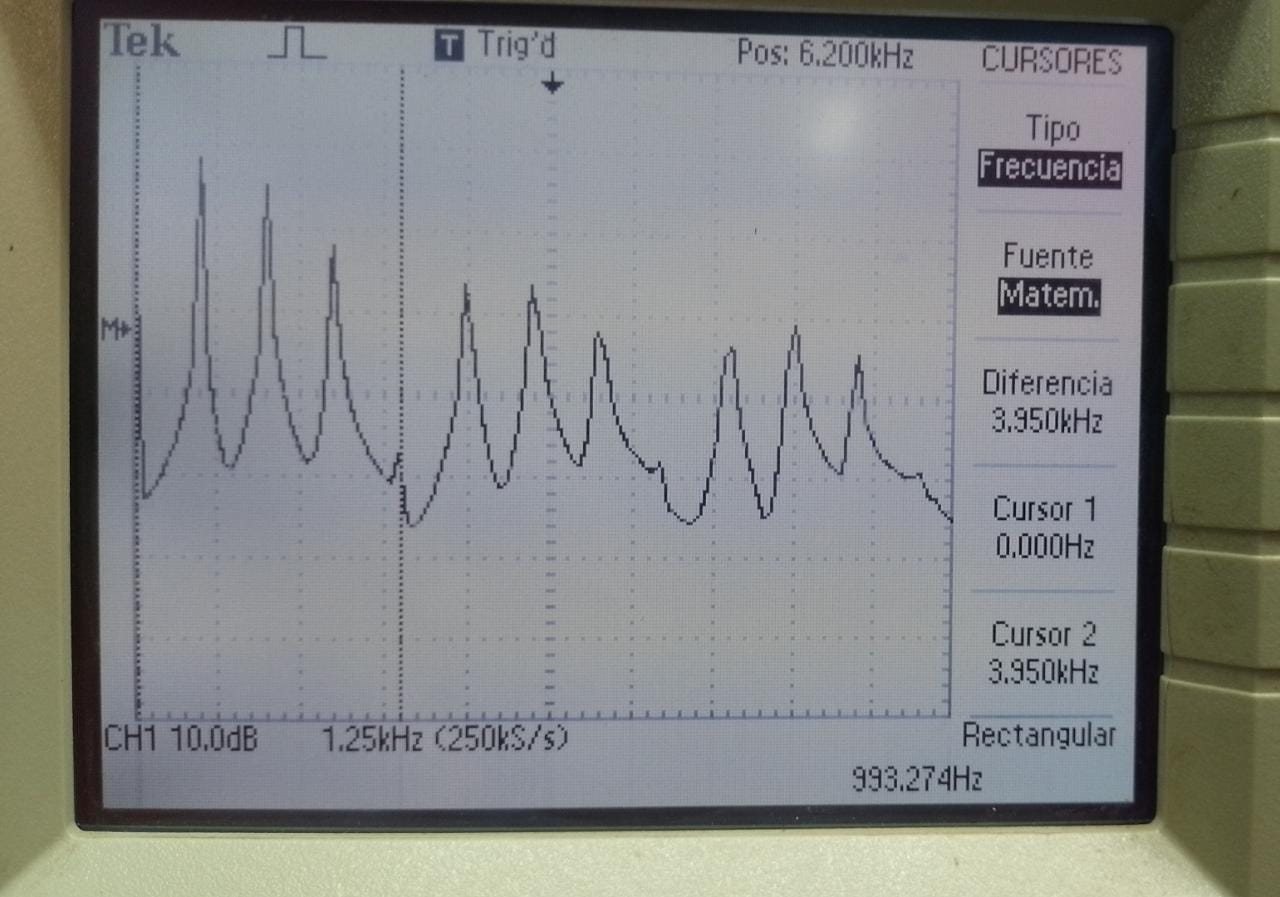
\includegraphics[width=\textwidth]{Imagenes/ActividadPractica/2AnalisisDeUnTrenDePulsos/Exp2_FrecArmonico4.jpeg}}
          \caption{Frecuencia de la cuarta armónica en ventana Rectangular, $f_{4}=3950~Hz$.}
        \end{subfigure}
        \begin{subfigure}[H]{0.48\textwidth}
          \frame{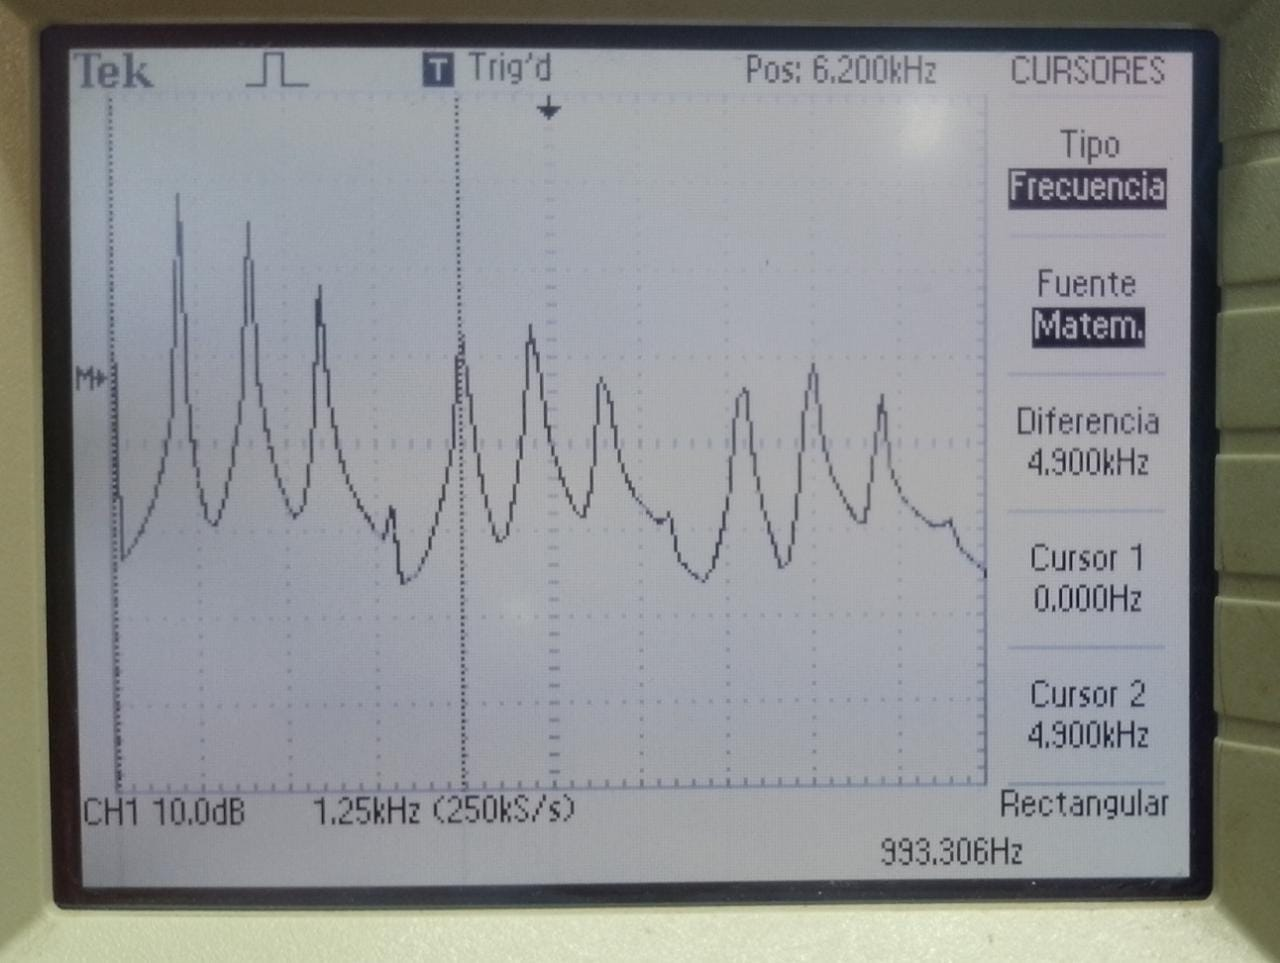
\includegraphics[width=\textwidth]{Imagenes/ActividadPractica/2AnalisisDeUnTrenDePulsos/Exp2_FrecArmonico5.jpeg}}
          \caption{Frecuencia de la quinta armónica en ventana Rectangular, $f_{5}=4900~Hz$.}
        \end{subfigure}

        \caption{Medición de frecuencia de picos de la señal pulsante en ventana Rectangular.}
        \label{fig:Exp2SeñalPulsanteArmonicosEspectro}
      \end{figure}     

      Se confecciona una tabla con las \textbf{diferencias de frecuencia} entre picos, en 
      base a las mediciones realizadas. Los valores se encuentran en la 
      Tabla~\ref{tab:Exp2MedicionesHanning}.

      \begin{table}[H]
      \centering
        \begin{tabular}{cccccc} \hline \hline
          \textbf{Cursor 2}               &  $\mathbf{1erArm.}$       & $\mathbf{2daArm.}$        & $\mathbf{3raArm.}$  &   $\mathbf{4taArm.}$ &   $\mathbf{5taArm.}$ \\ \hline
          $\mathbf{\Delta f_{n}~[Hz]}$     &   $950$                   &    $1000$                  &   $1000$             & $1000$                & $950$                \\ \hline \hline
         \end{tabular}
          \caption{Valores de frecuencia medidos en ventana Hanning.}
          \label{tab:Exp2MedicionesHanning}
      \end{table}

      Se calcula el promedio de las frecuencias como sigue
      \begin{align*}
        \Delta f_{n_{prom}}=\dfrac{\sum{\Delta_{fn}}}{n} \hspace{20pt} \therefore \hspace{20pt} \boxed{\Delta_{fn_{prom}}=980~[Hz]}~,
      \end{align*}
      y el período de la onda de pulsos es 
      \begin{align*}
        Periodo~\left( T \right)=\dfrac{1}{\Delta f_{n_{prom}}} \hspace{20pt} \therefore \hspace{20pt} \boxed{Periodo~\left( T \right)=1,02~[ms]}~.
      \end{align*}

        Se repite el experimento utilizando la ventana \textbf{Flattop}, pero ésta vez se miden los 
        \textbf{valles} que presenta el espectro, que se visualiza en la 
        Figura~\ref{fig:Exp2SeñalPulsanteVallesEspectro}.

       \begin{figure}[H]
        \centering
        \begin{subfigure}[H]{0.48\textwidth}
          \frame{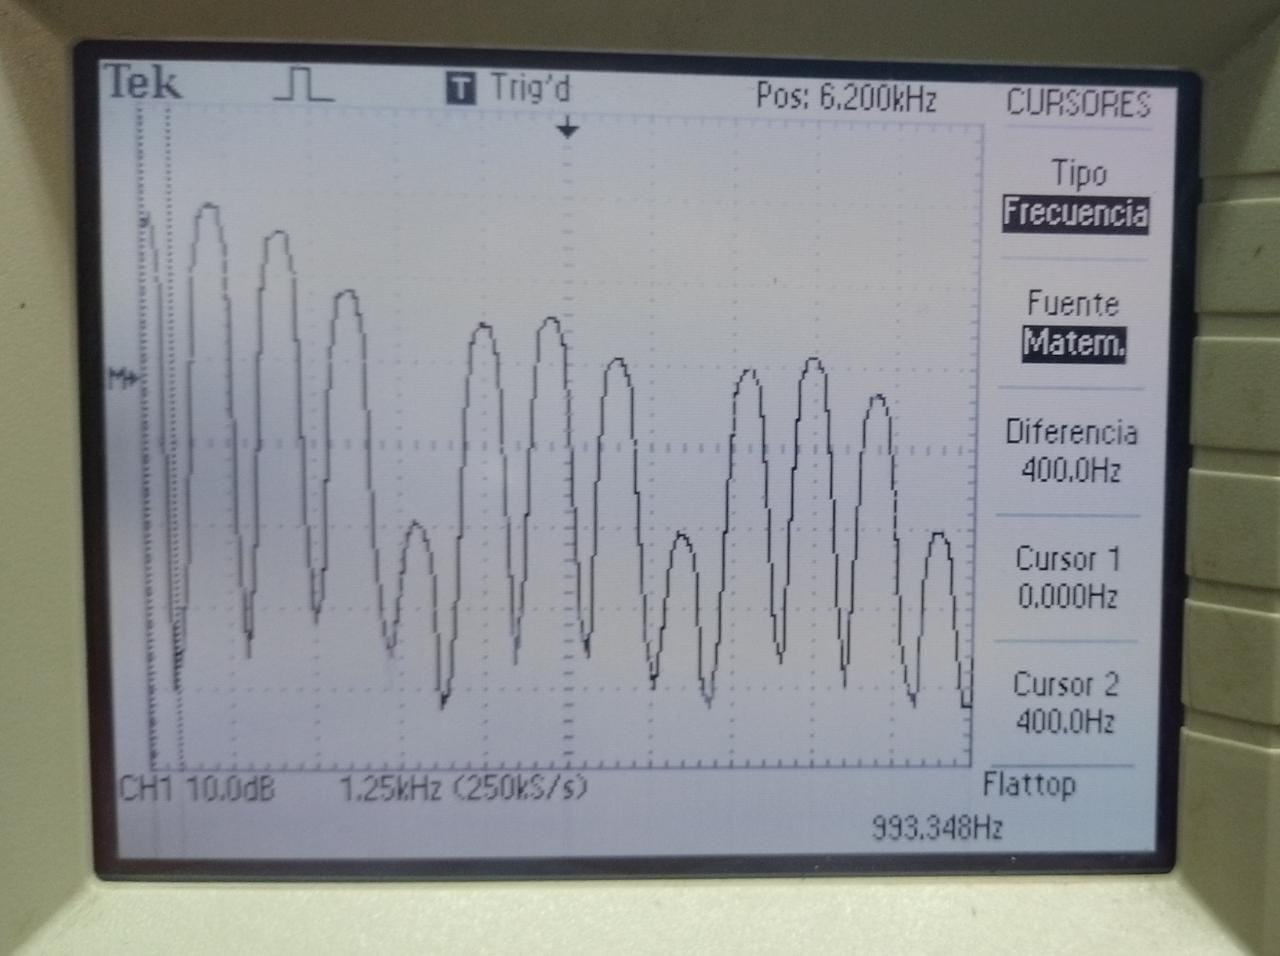
\includegraphics[width=\textwidth]{Imagenes/ActividadPractica/2AnalisisDeUnTrenDePulsos/Exp2_FrecValle1Flattop.jpeg}}
          \caption{Frecuencia del primer valle en ventana Flattop, $f_{a}=400~Hz$.}
        \end{subfigure}
        \hfill
        \begin{subfigure}[H]{0.48\textwidth}
          \frame{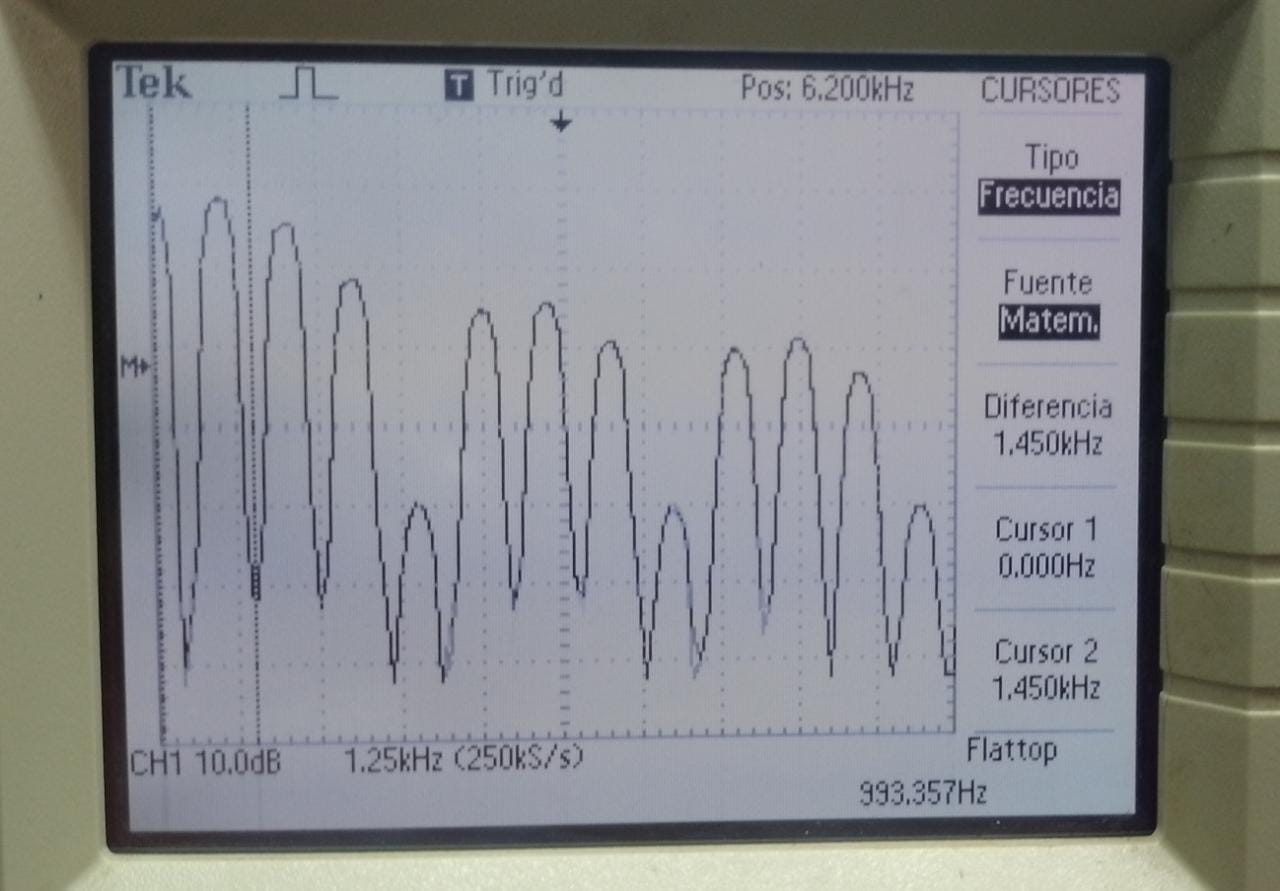
\includegraphics[width=\textwidth]{Imagenes/ActividadPractica/2AnalisisDeUnTrenDePulsos/Exp2_FrecValle2Flattop.jpeg}}
          \caption{Frecuencia del segundo valle en ventana Flattop, $f_{b}=1450~Hz$.}
        \end{subfigure}
        \hfill
        \begin{subfigure}[H]{0.48\textwidth}
          \frame{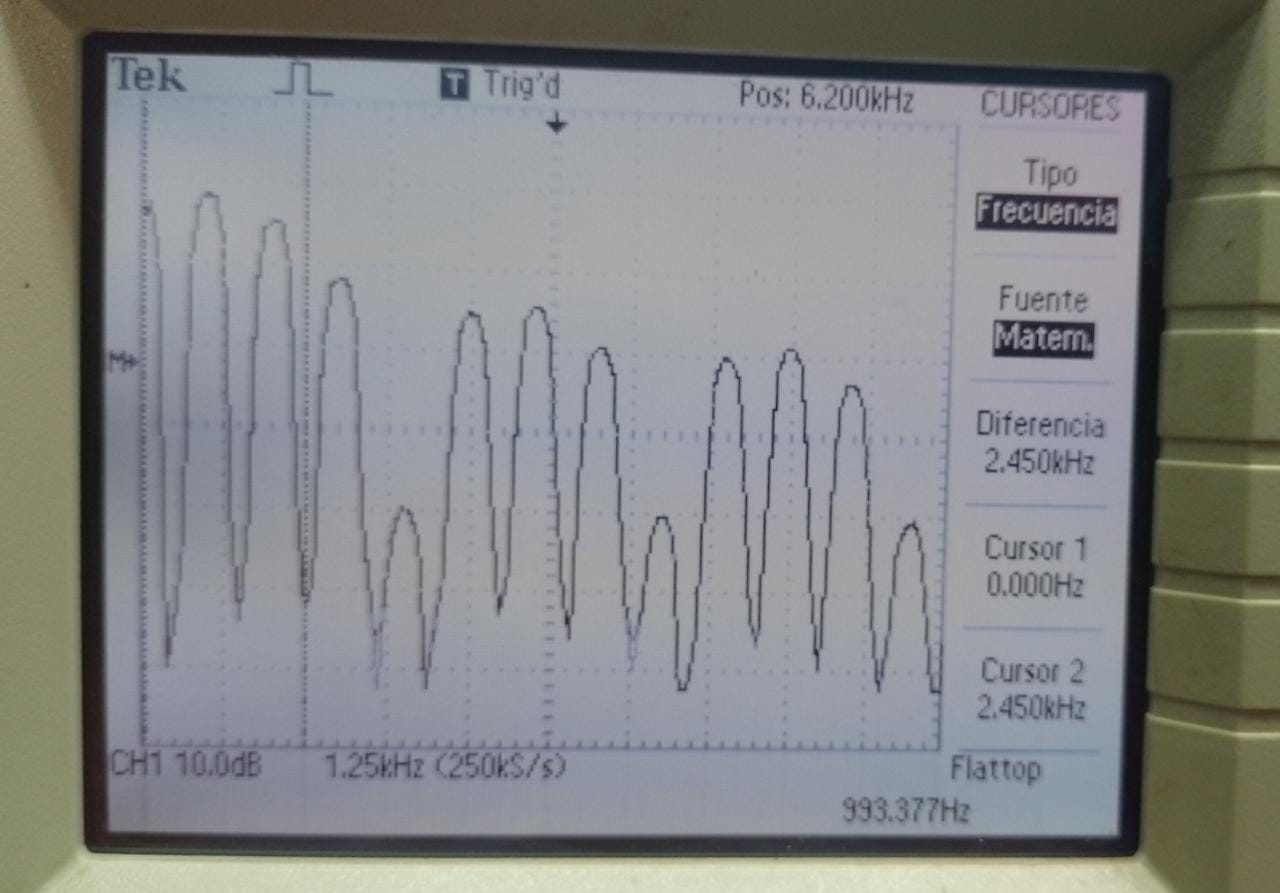
\includegraphics[width=\textwidth]{Imagenes/ActividadPractica/2AnalisisDeUnTrenDePulsos/Exp2_FrecValle3Flattop.jpeg}}
          \caption{Frecuencia del tercer valle en ventana Flattop, $f_{c}=2450~Hz$.}
        \end{subfigure}

        \caption{Medición de frecuencia de valles de la señal pulsante en ventana Flattop.}
        \label{fig:Exp2SeñalPulsanteVallesEspectro}
      \end{figure}     

      Se confecciona una tabla con los valores obtenidos, los mismos se encuentran en la 
      Tabla~\ref{tab:Exp2MedicionesFlattop}, y se calculan nuevamente el $\Delta f_{n_{prom}}$
      y el período. 

      \begin{table}[H]
      \centering
        \begin{tabular}{ccc} \hline \hline
          $\mathbf{\Delta_{fmin1}}$               &  $\mathbf{\Delta_{fmin2}}$       & $\mathbf{\Delta_{fmin3}}$ \\ \hline
                    $400~Hz$                        &    $1050~Hz$                    &   $1000~Hz$  \\ \hline \hline
         \end{tabular}
          \caption{Valores de frecuencia medidos en ventana Flattop.}
          \label{tab:Exp2MedicionesFlattop}
      \end{table}  

      \begin{align*}
        \Delta_{fn_{prom}}=\dfrac{\sum{\Delta_{fn}}}{n} \hspace{20pt} \therefore \hspace{20pt} \boxed{\Delta_{fn_{prom}}=816,67~[Hz]}
      \end{align*}        

      \begin{align*}
        Periodo~\left( T \right)=\dfrac{1}{\Delta_{fn_{prom}}} \hspace{20pt} \therefore \hspace{20pt} \boxed{Periodo~\left( T \right)=1,224~[ms]}
      \end{align*}

      Finalmente, se mide la amplitud de la frecuencia correspondiente a $0~Hz$, y se mide 
      también con multímetro el nivel de continua de la señal, posteriormente se comparan 
      los resultados.

       \begin{figure}[H]
        \centering
        \begin{subfigure}[H]{0.48\textwidth}
          \frame{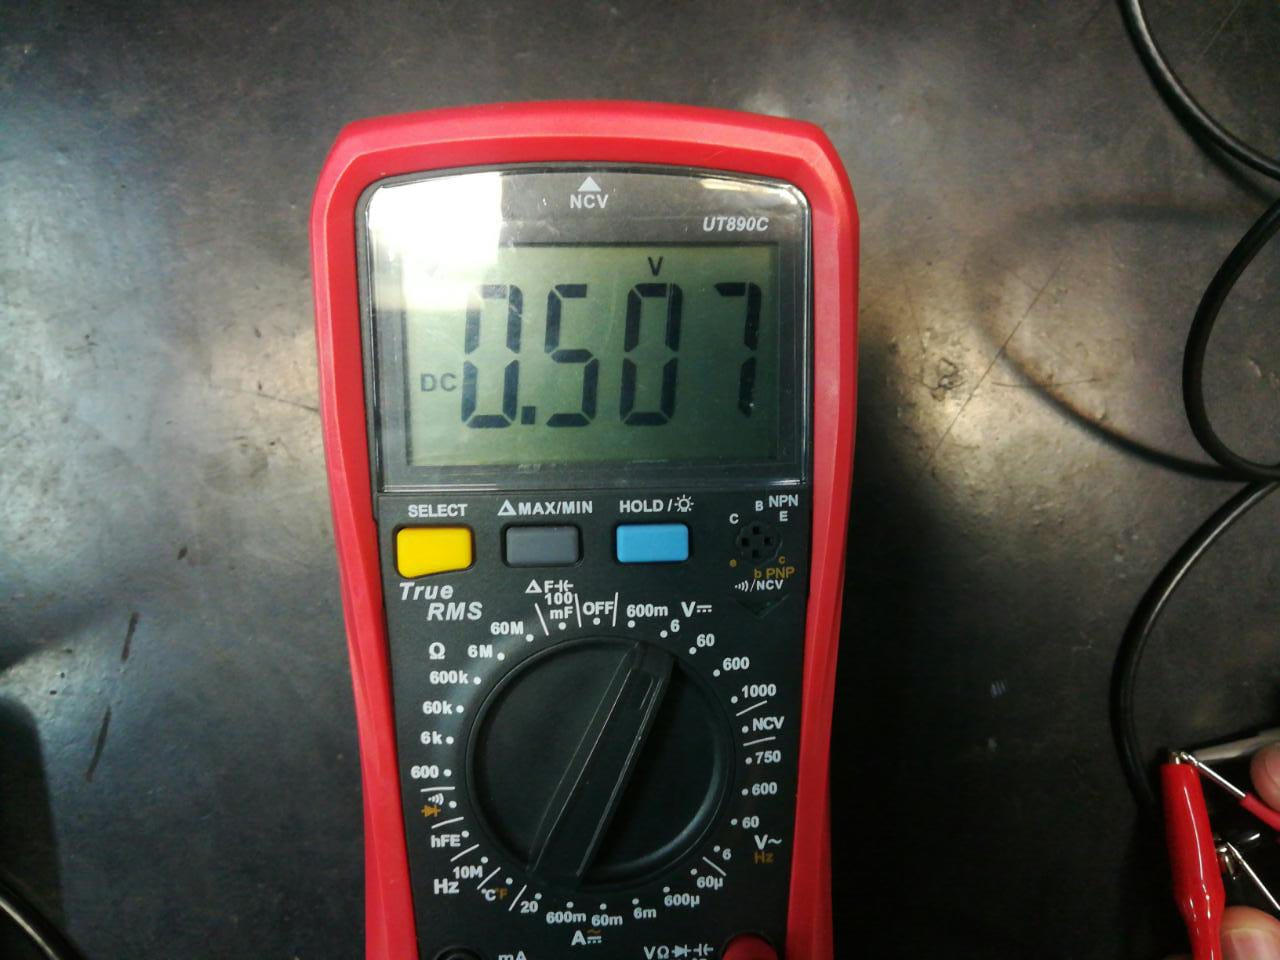
\includegraphics[width=\textwidth]{Imagenes/ActividadPractica/2AnalisisDeUnTrenDePulsos/MedicionCCOscilo.jpeg}}
          \caption{Medición de continua con osciloscopio, $CC_{osc}=1~V$.}
        \end{subfigure}
        \hfill
        \begin{subfigure}[H]{0.48\textwidth}
          \frame{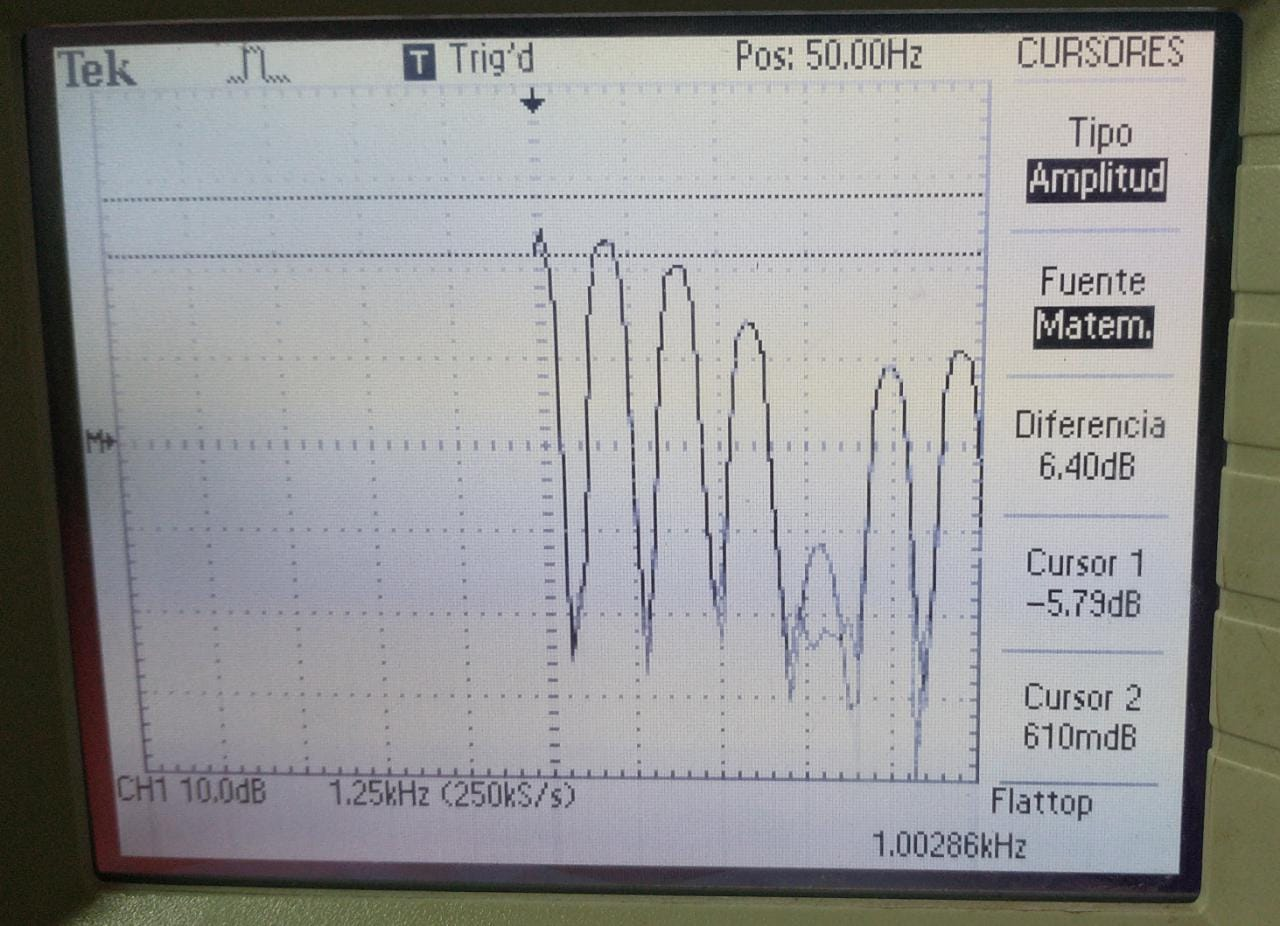
\includegraphics[width=\textwidth]{Imagenes/ActividadPractica/2AnalisisDeUnTrenDePulsos/MedicionCCMultiM.jpeg}}
          \caption{Medición de continua con multímetro, $CC_{Mult}=1~V$.}
        \end{subfigure}

        \caption{Medición del nivel de continua de la señal pulsante.}
        \label{fig:Exp2SeñalPulsanteContinua}
      \end{figure}        

      La medición realizada con el osciloscopio da como resultado $V_{rms}=0,513~V$, lo cual coincide con la medición realizada
      con el multímetro.


      \subsection{Obervación de frecuencias producto del aliasing}

    \input{Secciones/Subsecciones/4AnalisisDeUnaSeñalDeAM.tex}
      \subsection{Observación de los productos de IMD de tercer orden}
    En la experiencia anterior se hace uso de un diodo para poder generar la modulación de
    amplitud. El circuito en cuestión se puede ver en la Figura~\ref{fig:ModuladorAM} de
    la Sección~\ref{sec:Exp4_AM}.

    Este dispositivo tiene un comportamiento alineal, el cual se puede modelar
    de la siguiente  forma

    \vspace{-10pt}
    \begin{equation*}
      v_{AM} = k_a(v_{G1}+v_{G2}) + k_b(v_{G1}+v_{G2})^2 + k_c(v_{G1}+v_{G2})^3 + \cdots
    \end{equation*}
    donde es de especial interés la región cuadrática de este dispositivo, ya que,
    debido a este, se obtiene la modulación de amplitud buscada. Si se 
    desarrolla el término correspondiente (el cuadrático), se logra justificar lo
    mencionado
    
    \vspace{-10pt}
    \begin{equation*}
      v_{AM} = \cdots + k_b(v_{G1}^2 + 2\cdot{v_{G1}v_{G2}} + v_{G2}^2) + \cdots ~.
    \end{equation*}

    Por el contrario, las \textbf{alinealidades de orden superior} dan como resultado \textbf{productos
    de intermodulación} (\textbf{IMD}), los cuales son efectos no deseados. La alinealidad más
    importante suele ser la IMD de tercer orden, por lo cual, ahora se procede a determinar el
    \textbf{rechazo de IMD de tercer orden} del circuito modulador utilizado.

    Para ello, se setean ambos generadores \textbf{G1} y \textbf{G2} a una frecuencia de 
    \textbf{f=50~kHz}, y a \textbf{igual amplitud}. Luego, se observan las señales de salida del circuito 
    dejando un solo generador encendido. Los resultados se encuentran en las Figuras~\ref{fig:SalidaCircuitConG1Encendido}
    y \ref{fig:SalidaCircuitConG2Encendido}.


    \begin{figure}[H]
      \centering
      \begin{subfigure}[H]{0.48\textwidth}
        \frame{\includegraphics[width=\textwidth]{Imagenes/ActividadPractica/5ProductosDeIMPde3erOrden/Exp5_SeñalSalidaConG1Autoset_Tiempo.jpeg}}
        \caption{En tiempo.}
      \end{subfigure}
      \hfill 
      \begin{subfigure}[H]{0.48\textwidth}
        \frame{\includegraphics[width=\textwidth]{Imagenes/ActividadPractica/5ProductosDeIMPde3erOrden/Exp5_SeñalSalidaConG1_Frecuencia.jpeg}}
        \caption{En frecuencia.}
      \end{subfigure}

      \caption{Salida del circuito con el generador G1 encendido.}
      \label{fig:SalidaCircuitConG1Encendido}
    \end{figure}


    \begin{figure}[H]
      \centering
      \begin{subfigure}[H]{0.48\textwidth}
        \frame{
\includegraphics[width=\textwidth]{Imagenes/logo-utn.png}}
        \caption{En tiempo.}
      \end{subfigure}
      \hfill 
      \begin{subfigure}[H]{0.48\textwidth}
        \frame{\includegraphics[width=\textwidth]{Imagenes/ActividadPractica/5ProductosDeIMPde3erOrden/Exp5_SeñalSalidaConG2_Frecuencia.jpeg}}
        \caption{En frecuencia.}
      \end{subfigure}

      \caption{Salida del circuito con el generador G2 encendido.}
      \label{fig:SalidaCircuitConG2Encendido}
    \end{figure}

    A continuación, se encienden ambos generadores y se ajusta el tiempo de muestreo y se habilita el \textbf{Zoom x10}
    para obtener una mejor visualización. Luego, se procede a separar ambas señales un ancho de $\mathbf{\triangle f=  2~kHz}$,
    quedando una de ellas en $\mathbf{f_1=49~kHz}$ y la otra en $\mathbf{f_2=51~kHz}$. En la
    Figura~\ref{fig:SalidaConAmbosGeneradores} se puede ver lo explicado en este párrafo.

    \begin{figure}[H]
      \centering
      \begin{subfigure}[H]{0.48\textwidth}
        \frame{\includegraphics[width=\textwidth]{Imagenes/ActividadPractica/5ProductosDeIMPde3erOrden/Exp5_SeñalSalidaConLosDosGeneradores_Frec.jpeg}}
        \caption{Ambas a la misma frecuencia.}
      \end{subfigure}
      \hfill 
      \begin{subfigure}[H]{0.48\textwidth}
        \frame{\includegraphics[width=\textwidth]{Imagenes/ActividadPractica/5ProductosDeIMPde3erOrden/Exp5_SeparacionDeSeñalesDe2KHz.jpeg}}
        \caption{Con separación de $2~kHz$.}
      \end{subfigure}

      \caption{Espectro de la señal de salida con ambas señales inyectadas al circuito.}
      \label{fig:SalidaConAmbosGeneradores}
    \end{figure}

    Las componentes de $\mathbf{47~kHz}\  (2f_1 - f2)$ y $\mathbf{53~kHz}\  (2f_2 - f1)$ son los productos de IMD de tercer orden. Para obtenerlos
    se realiza la diferencia en amplitud entre estas y \textbf{f\textsubscript{1}} y \textbf{f\textsubscript{2}} respectivamente. Dichas mediciones,
    realizadas con la ventana \textbf{Hanning}, se pueden ver en la Figura~\ref{fig:MedicionIMD}.

    \begin{figure}[H]
      \centering
      \begin{subfigure}[H]{0.48\textwidth}
        \frame{\includegraphics[width=\textwidth]{Imagenes/ActividadPractica/5ProductosDeIMPde3erOrden/Exp5_IDM3erOrdenConSeñal49kHz.jpeg}}
        \caption{Para $f_1=49~kHz$.}
      \end{subfigure}
      \hfill 
      \begin{subfigure}[H]{0.48\textwidth}
        \frame{\includegraphics[width=\textwidth]{Imagenes/ActividadPractica/5ProductosDeIMPde3erOrden/Exp5_IDM3erOrdenConSeñal51kHz.jpeg}}
        \caption{Para $f_2=51~kHz$.}
      \end{subfigure}

      \caption{Medición de diferencia de amplitudes.}
      \label{fig:MedicionIMD}
    \end{figure}

    Los valores obtenidos de esta experiencia se encuentran tabulados en la Tabla~\ref{tab:DatosDeMedicionDeIMD}.

    \begin{table}[H]
      \centering
    \begin{tabular}{ccccc} \hline \hline
      $\mathbf{f_{1}}$    &   $\mathbf{f_{2}}$  &  $\mathbf{2f_{1}-f_{2}}$  & $\mathbf{2f_{2}-f_1}$  & \textbf{Rechazo IMD 3º}\\ \hline
      $49~kHz$   &   $51~kHz$   &    $47~kHz$   &   $53~kHz$  & $15,2~dB$ \\ \hline \hline
      \end{tabular}
      \caption{Valores obtenidos para la medición del rechazo de IMD de 3º.}
      \label{tab:DatosDeMedicionDeIMD}
    \end{table}


    \pagebreak



    \input{Secciones/Subsecciones/6AnalisisDeUnaSeñalDeFM.tex}
      \subsection{Análisis de la distorsión armónica producida por un amplificador}

